% !TEX root = ../../../main.tex
% 来源：中学数学实验教材·第三册（高中数学）
% 章节：任意角的三角函数 / 三角函数的诱导公式
% 原始文件：6.tex，行 1927-1939
% 类型：tikz
% ---
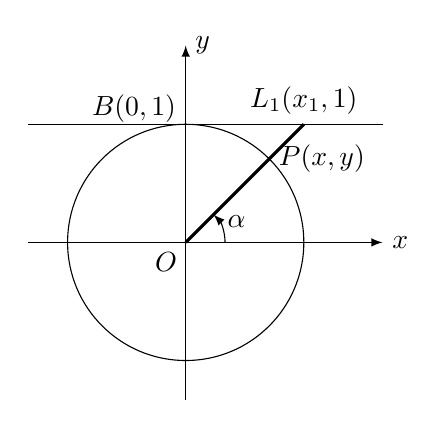
\begin{tikzpicture}[>=latex, scale=1]
    \draw[->](-2,0)--(2.5,0)node[right]{$x$};
    \draw[->](0,-2)--(0,2.5)node[right]{$y$};
    \draw (0,0) circle(1.5);
    \draw  (-2,1.5)--(2.5,1.5);
    \draw[very thick](0,0)--(1.5,1.5);
    \draw[->](.5,0) arc (0:45:.5);
    \node at (22.5:.7){$\alpha$};
\node at (-.25,-.25){$O$};
\node at (0,1.7)[left]{$B(0,1)$};
\node at (1.5,1.5)[above]{$L_1(x_1,1)$};
\node at (45:1.5)[right]{$P(x,y)$};
    \end{tikzpicture}
